\documentclass[9pt,xcolor={table}]{beamer}
\setbeamertemplate{caption}[numbered]
\usetheme[white]{Illinois}
%\title[short title]{long title}
\title[HALEU Transitions]{Investigation of Impacts of Deploying 
Reactors Fueled by High Assay Low Enriched Uranium}
\subtitle{Final Defense}
\author[Amanda M. Bachmann]{Amanda M. Bachmann\\ Advanced Reactors and Fuel Cycles Group}
%\author[Kathryn D. Huff]{Kathryn D. Huff\\Advanced Reactors and Fuel Cycles Group}
\date[11.02.2023]{November 2, 2023}
\institute[UIUC]{University of Illinois at Urbana-Champaign}


\usepackage[table]{xcolor}
\usepackage{amsfonts}
\usepackage{amsmath}
\usepackage{xspace}
\usepackage{graphicx}
\usepackage{caption}
\usepackage{subcaption}
\usepackage{booktabs} % nice rules for tables
\usepackage{microtype} % if using PDF
\usepackage{bigints}
\usepackage{array}
\newcolumntype{x}[1]{>{\centering\arraybackslash\hspace{0pt}}p{#1}}

\usepackage{threeparttable}

\graphicspath{{../images/}}

\newcommand{\units}[1] {\:\text{#1}}%
\newcommand{\SN}{S$_N$}%{S$_\text{N}$}%{$S_N$}%
\newcommand{\Cyclus}{\textsc{Cyclus}\xspace} %
\newcommand{\Cycamore}{\textsc{Cycamore}\xspace} %
\newcommand{\keff}{$k_{eff}$\xspace}
\newcommand{\betaEff}{$\beta_{eff}$\xspace}
\DeclareMathOperator{\erf}{erf}
%I need some complimentary error functions... 
\DeclareMathOperator{\erfc}{erfc}
%Those icons in the references are terrible looking
\setbeamertemplate{bibliography item}[text]

%%%% Acronym support

\usepackage[acronym,toc]{glossaries}
\input{../acros}

\usepackage{tikz}
\usetikzlibrary{shapes.geometric, arrows, backgrounds}
\usetikzlibrary{positioning, arrows, decorations, shapes, matrix, fit, tikzmark}

\tikzstyle{agent} = [rectangle, rounded corners, minimum width=0.1cm, minimum height=0.2cm,text centered, draw=black, fill=blue!30]
\tikzstyle{transition} = [rectangle, rounded corners, minimum width=0.1cm, minimum height=0.2cm,text centered, draw=black, fill=red!30]
\tikzstyle{arrow} = [thick,->,>=stealth]

\tikzstyle{region} = [rectangle, rounded corners, minimum width=0.1cm, minimum height=0.2cm,text centered, draw=black, fill=green!30]
\tikzstyle{institution} = [rectangle, rounded corners, minimum width=0.1cm, minimum height=0.2cm,text centered, draw=black, fill=red!30]
\tikzstyle{facility} = [rectangle, rounded corners, minimum width=0.1cm, minimum height=0.2cm,text centered, draw=black, fill=blue!30]
\tikzstyle{connect} = [thick,-]

\def\firstcircle{(0,0) circle (2cm)}
\def\secondcircle{(60:3cm) circle (2cm)}
\def\thirdcircle{(0:3cm) circle (2cm)}
\makeglossaries

%try to get rid of header on title page\dots
\makeatletter
    \newenvironment{withoutheadline}{
        \setbeamertemplate{headline}[default]
        \def\beamer@entrycode{\vspace*{-\headheight}}
    }{}
\makeatother

\makeatother
\setbeamertemplate{footline}
{
  \leavevmode%
  \hbox{%
    \rightline{\insertframenumber{} / \inserttotalframenumber\hspace*{1ex}}
  }%
  \vskip0pt%
}
\makeatletter
\begin{document}
%%%%%%%%%%%%%%%%%%%%%%%%%%%%%%%%%%%%%%%%%%%%%%%%%%%%%%%%%%%%%
%% From uw-beamer Here's a handy bit of code to place at 
%% the beginning of your presentation (after \begin{document}):
\newcommand*{\alphabet}{ABCDEFGHIJKLMNOPQRSTUVWXYZabcdefghijklmnopqrstuvwxyz}
\newlength{\highlightheight}
\newlength{\highlightdepth}
\newlength{\highlightmargin}
\setlength{\highlightmargin}{2pt}
\settoheight{\highlightheight}{\alphabet}
\settodepth{\highlightdepth}{\alphabet}
\addtolength{\highlightheight}{\highlightmargin}
\addtolength{\highlightdepth}{\highlightmargin}
\addtolength{\highlightheight}{\highlightdepth}
\newcommand*{\Highlight}{\rlap{\textcolor{HighlightBackground}{\rule[-\highlightdepth]{\linewidth}{\highlightheight}}}}
\colorlet{lightblue}{blue!40!}
\definecolor{lightorange}{HTML}{FAA21A}
\colorlet{lightpink}{red!20!}

\tikzset{   
        every picture/.style={remember picture,baseline},
        every node/.style={anchor=base,align=center,outer sep=1.5pt},
        every path/.style={thick},
        }

\newcommand\marktopleft[1]{%
    \tikz[overlay,remember picture] 
        \node (marker-#1-a) at (.1em,.3em) {};%
}
\newcommand\markbottomright[1]{%
    \tikz[overlay,remember picture] 
        \node (marker-#1-b) at (.1em,.3em) {};%
    \tikz[overlay,remember picture,inner sep=3pt]
        \node[draw=red,rounded corners,fit=(marker-#1-a.north west) (marker-#1-b.south east)] {};%
}

%%%%%%%%%%%%%%%%%%%%%%%%%%%%%%%%%%%%%%%%%%%%%%%%%%%%%%%%%%%%%
%%--------------------------------%%
\begin{withoutheadline}
    \frame{
      \titlepage
    }
    \end{withoutheadline}

%%--------------------------------%%
\AtBeginSection[]{
\begin{frame}
  \frametitle{Outline}
  \tableofcontents[currentsection]
\end{frame}
}


\section{Introduction}
\subsection{Motivation}
\begin{frame}
    \frametitle{The US is looking to develop supplies of HALEU}
    \begin{columns}
        \column[t]{5cm}
    \begin{itemize}
    \item Multiple new reactor designs require \gls{HALEU} fuel, which allows for: 
    \begin{itemize}
        \item Longer cycle time
        \item Increased capacity factor
        \item Higher burnup 
    \end{itemize}
    \item<2-> The US does not have any commercial supplies of \gls{HALEU}
    \item<3-> To meet the \gls{HALEU} demand, the U.S. \gls{DOE} has proposed two methods \cite{griffith_overview_2020}:
    \begin{itemize}
        \item Enrichment of natural uranium
        \item Recovery and downblending of \gls{HEU}
    \end{itemize}
    
    \end{itemize}

    \column[t]{5cm}
    \begin{table}
        \centering
        \caption{Categories of uranium enrichment by weight fraction of 
        $^{235}$U.}
        \label{tab:enrichemnt}
        \begin{tabular}{l c c}
            \hline
            Category & Weight fraction (\%)\\\hline
            Depleted & $<$0.711 \\
            Natural & 0.711 \\
            LEU & 0.711-20 \\
            \gls{HALEU} & 5-20 \\
            \gls{HEU} & $\ge$20 \\
            \hline
        \end{tabular}
    \end{table}
    \end{columns}
\end{frame}

\subsection{Background}
\begin{frame}
    \frametitle{Nuclear fuel cycle}
    \begin{figure}
    \centering
    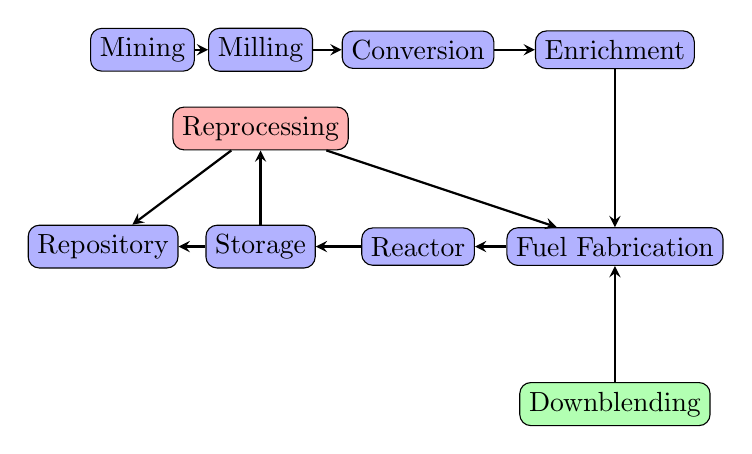
\begin{tikzpicture}[node distance=1cm]
        \node (mine) [agent] {Mining};
        \node (mill) [agent, right of=mine, xshift=0.5cm] {Milling};
        \node (conversion) [agent, right of=mill, xshift=1cm] {Conversion};
        \node (enrichment) [agent, right of=conversion, xshift=1.5cm]{Enrichment};
        \node (fabrication) [agent, below of=enrichment, yshift=-1.5cm]{Fuel Fabrication};
        \node (reactor) [agent, left of=fabrication, xshift=-1.5cm]{Reactor};
        \node (storage) [agent,  left of=reactor, xshift=-1cm]{Storage};
        \node (sinkhlw) [agent, left of=storage, xshift=-1cm]{Repository};


        \draw [arrow] (mine) --  (mill); 
        \draw [arrow] (mill) -- (conversion); 
        \draw [arrow] (conversion) -- (enrichment);
        \draw [arrow] (enrichment) -- (fabrication);
        \draw [arrow] (fabrication) -- (reactor);
        \draw [arrow] (reactor) -- (storage);
        \draw [arrow] (storage) -- (sinkhlw);
        \pause
        \node (reprocessing) [transition, above of=storage, yshift=0.5cm]{Reprocessing};
        
        \draw [arrow] (storage) -- (reprocessing);
        \draw [arrow] (reprocessing) -- (fabrication);
        \draw [arrow] (reprocessing) -- (sinkhlw);
        \pause
        \node (downblending) [region, below of=fabrication, yshift=-1cm]{Downblending};
        \draw [arrow] (downblending) -- (fabrication);

        \end{tikzpicture}
    \caption{Overview of the Nuclear Fuel Cycle.}
    \label{fig:fuel_cycle}
\end{figure}
\end{frame}

\begin{frame}
    \frametitle{Uranium enrichment}
    \begin{itemize}
        \item Process to increase the relative abundance of specific
              isotopes of an element
        \pause
        \item The throughput of a facility is based on the product 
              mass, product assay, and the \gls{SWU} capacity
    \end{itemize}
    \pause
    \vspace{-0.2cm}
    \begin{columns}
        \column{6.5cm}
            \begin{align*}
                    & F = P + T \\
                    & x_fF = x_pP + x_tT\\
                    & SWU = \left[P\times V(x_p) +T*V(x_t) - F*V(x_f)\right]*t\\
                    & \text{in which:}\\
                    & V(x_i) = (2x_i - 1)*\ln\left(\frac{x_i}{1-x_i}\right)
            \end{align*}
            \vspace{-0.5cm}
            \begin{figure}[t]
    \centering
    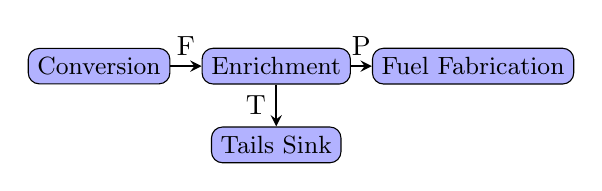
\begin{tikzpicture}[node distance=1cm]
        \node (conversion) [agent] {\small Conversion};
        \node (enrichment) [agent, right of=conversion, xshift=1.25cm]{\small Enrichment};
        \node (fabrication) [agent, right of=enrichment, xshift=1.5cm]{\small Fuel Fabrication};
        \node (sink) [agent, below of=enrichment]{\small Tails Sink};
        
        \draw [arrow] (conversion) -- node[anchor=south]{F} (enrichment);
        \draw [arrow] (enrichment) -- node[anchor=south]{P}(fabrication);
        \draw [arrow] (enrichment) -- node[anchor=east]{T}(sink);

        \end{tikzpicture}
\end{figure}
    \column{3.5cm}
    \begin{table}
        \centering
        \vspace{-0.3cm}
        \begin{tabular}{c m{2cm}}
            \hline
            Variable & Definition \\
            \hline
            F & feed mass \\
            P & product mass \\
            T & tails mass\\
            x$_i$ & assay of material stream \\
            SWU & Separative Work Units\\
            V(x$_i$) & separation potential function\\
            \hline
        \end{tabular}
    \end{table}

    \end{columns}
\end{frame}

\begin{frame}
    \frametitle{Efforts to estimate HALEU needs}
    Efforts are underway to estimate potential \gls{HALEU} needs:
    \begin{itemize}
        \item \gls{NEI} surveyed multiple reactor design companies
              to estimate \gls{HALEU} needs between now and 2035 
              \cite{korsnick_updated_2021,nuclear_energy_institute_establishing_2022}
        \item \gls{DOE} labs modeled the transition to some 
              \gls{HALEU}-fueled reactors to estimate \gls{HALEU} needs 
              to meet current net-zero carbon goals in 2050 \cite{dixon_estimated_2022}
    \end{itemize}
    This previous work is all based on announced advanced reactor projects.
\end{frame}

\subsection{Objectives}
\begin{frame}
    \frametitle{Technical gaps \& objectives}
    \begin{block}{Technical Gaps}
        \begin{itemize}
            \item Understand changes to the US nuclear fuel cycle to 
                  commercially supply \gls{HALEU}
            \item Understand limitations of using downblended \gls{HEU} 
                  in advanced reactors         
        \end{itemize}
    \end{block}
    \pause
    \begin{block}{Objectives}
        \begin{itemize}
        \item<2-> Explore how the deployment of \gls{HALEU}-fueled reactors 
        affects the US nuclear fuel cycle. 
        \item<2-> Quantify potential material requirements for the transition from 
              \glspl{LWR} to advanced reactors in a once-through and recycling 
              fuel cycle
        \item<2-> Understand the impacts of fuel cycle parameters on the 
              material requirements and design optimized transition scenarios
        \item<2-> Identify potential limitations in using downblended \gls{HEU} 
              in advanced reactors
        \end{itemize}
    \end{block}
\end{frame}
\section{Transition analysis}
\begin{frame}
    \frametitle{Transition analysis}
    To meet the first objective, I model the transition from the current 
    \gls{LWR} fleet to advanced reactors
    \begin{itemize}
        \item Use fuel cycle simulators to model the transition
        \item Model the deployment and decommissioning of fuel cycle facilities 
        \item Model material transactions between facilities
        \item Quantify material requirements to understand potential \gls{HALEU}
              demand
    \end{itemize}

\end{frame}

\subsection{Once-through fuel cycles}
\begin{frame}
    \frametitle{Transition analysis assumptions}
    \begin{columns}
        
    \column[t]{6cm}
    \vspace{-0.9cm}
    \begin{figure}[t]
    \centering
    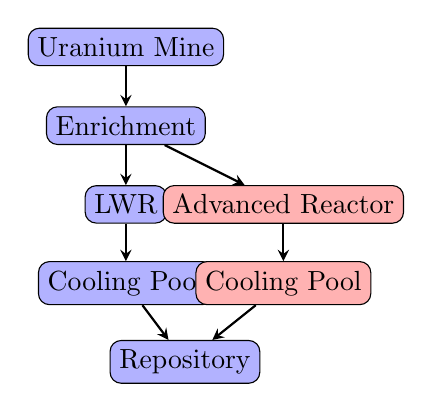
\begin{tikzpicture}[node distance=1cm]
        \node (mine) [agent] {Uranium Mine};
        \node (enrichment) [agent, below of=mine]{Enrichment};
        \node (reactor) [agent, below of=enrichment]{LWR};
        \node (adv_reactor) [transition, below of=enrichment, xshift=2cm]{Advanced Reactor};
        \node (wetstorage) [agent, below of=reactor]{Cooling Pool};
        \node (sinkhlw) [agent, below of=wetstorage, xshift=0.75cm]{Repository};
        \node (adv_rx_cooling) [transition, below of=adv_reactor]{Cooling Pool};

        \draw [arrow] (mine) --  (enrichment); 
        \draw [arrow] (enrichment) -- (reactor);
        \draw [arrow] (enrichment) -- (adv_reactor);
        \draw [arrow] (reactor) -- (wetstorage);
        \draw [arrow] (wetstorage) -- (sinkhlw);
        \draw [arrow] (adv_reactor) -- (adv_rx_cooling);
        \draw [arrow] (adv_rx_cooling) -- (sinkhlw);
        \end{tikzpicture}
    \caption{Fuel cycle facilities and material flow between facilities. Facilities 
    in red are deployed at the start of the transition. }
    \label{fig:fuel_cycle}
\end{figure}

        \column[t]{4.5cm}
        Model transitions using \Cyclus \cite{huff_fundamental_2016}
        \begin{itemize}
            \item Simulations model reactor deployment from 1965-2090
            \item Transitions begin in 2025
            \item<2-> \gls{LWR} commission dates are obtained from the IAEA PRIS
                database \cite{noauthor_power_1989}
            \item<2-> \glspl{LWR} are assumed to operate until their current license 
                expires
            \item<3-> Manually calculate advanced reactor deployment
            \item<3-> Assume natural uranium is enriched to produce all 
                  fuel
        \end{itemize}

\end{columns}
\end{frame}

\begin{frame}
    \frametitle{Advanced reactors}
    \vspace{-0.2cm}
    \begingroup
        \renewcommand{\arraystretch}{1.5}
        \begin{table}
            \small
            \caption{Advanced reactor design specifications}
            \label{tab:reactor_summary}
            \vspace{-0.15cm}
            \begin{tabular}{ l p{1.5cm} p{1.5cm} p{2cm} }
                \hline
                Design Criteria & USNC MMR 
                    \cite{noauthor_usnc_2021} & 
                    X-energy Xe-100 \cite{mulder_overview_2021} & 
                    NuScale VOYGR \cite{nuscale_chapter_2020-1,reyes_nuscale_2021,reyes_correction_2022}\\\hline
                Reactor type & HTGR & HTGR & SMR\\
                Fuel type & UO$_2$ FCM & UCO TRISO & UO$_2$ pellets \\
                Power (MWe) & 5 & 80 & 77\\
                Power (MWth) & 15 & 200 & 250\\
                Enrichment (\% $^{235}U$) & 19.75 & 15.5 & 4.09 \\
                Cycle Length (yr) & 20 & Online & 1.5 \\
                Number of cycles & 1 & 6 & 3\\
                Reactor Lifetime (yr) & 20 & 60 & 60\\
                Burnup ($\frac{MWd}{kg U}$) & 82 & 168 & 45\\
                \hline
            \end{tabular}
        \end{table}   
    \endgroup
    \begin{equation}
        \text{mass (kg)} = \frac{\text{Power (MWth) * cycle length (d)*number of cycles}}{\text{Burnup (MWd/kg)}}
        \label{eq:fuel_mass}
    \end{equation}
\end{frame}

\begin{frame}
    \frametitle{Once-through scenario definitions}
        \begin{table}[ht]
            \centering
            \caption{Summary of the once-through fuel cycle transition scenarios.
                     Energy growth is relative to energy from \glspl{LWR} in 2025.}
            \label{tab:scenarios_once-through}
            \begin{tabular}{c l l}
                    \hline
                    Scenario number & Reactors present & Energy demand\\\hline
                    \rowcolor{lightblue} 1 & \glspl{LWR} & N/A \\
                    \rowcolor{lightorange}2 & \glspl{LWR} and MMR & No growth \\
                    \rowcolor{lightorange}3 & \glspl{LWR} and Xe-100 & No growth \\
                    \rowcolor{lightorange}4 & \glspl{LWR}, Xe-100, and MMR& No growth\\
                    \rowcolor{lightorange}5 & \glspl{LWR}, MMR, and VOYGR & No growth\\
                    \rowcolor{lightorange}6 & \glspl{LWR}, Xe-100, and VOYGR & No growth\\
                    \rowcolor{lightorange}7 & \glspl{LWR}, Xe-100, MMR, and VOYGR & No growth\\
                    \rowcolor{lightpink}8 & \glspl{LWR} and MMR& 1\% growth \\
                    \rowcolor{lightpink}9 & \glspl{LWR} and Xe-100 & 1\% growth\\
                    \rowcolor{lightpink}10 & \glspl{LWR}, Xe-100, and MMR& 1\% growth\\
                    \rowcolor{lightpink}11 & \glspl{LWR}, MMR, and VOYGR & 1\% growth\\
                    \rowcolor{lightpink}12 & \glspl{LWR}, Xe-100, and VOYGR & 1\% growth\\
                    \rowcolor{lightpink}13 & \glspl{LWR}, Xe-100, MMR, and VOYGR & 1\% growth\\
                    \hline
            \end{tabular}
        \end{table}
        %<2-> \tikz[overlay, remember picture]{\draw{draw=red,thick, double, fillopacity=0.2] ($(infrastructure)+(-0.5,0.4)$) rectangle ($(infrastructure)+(6,-0.2)$);}} 
\end{frame}

\begin{frame}
    \frametitle{Once-through scenario definitions}
        \begin{table}[ht]
            \centering
            \caption{Summary of the once-through fuel cycle transition scenarios.
            Energy growth is relative to energy from \glspl{LWR} in 2025.}
            \label{tab:scenarios_once-through}
            \begin{tabular}{c l l}
                \hline
                Scenario number & Reactors present & Energy demand\\\hline
                \rowcolor{lightblue} 1 & \glspl{LWR} & N/A \\
                \rowcolor{lightorange}\marktopleft{a3}2 & \glspl{LWR} and MMR & No growth \\
                \rowcolor{lightorange}3 & \glspl{LWR} and Xe-100 & No growth \\
                \rowcolor{lightorange}4 & \glspl{LWR}, Xe-100, and MMR& No growth\\
                \rowcolor{lightorange}5 & \glspl{LWR}, MMR, and VOYGR & No growth\\
                \rowcolor{lightorange}6 & \glspl{LWR}, Xe-100, and VOYGR & No growth\\
                \rowcolor{lightorange}7 & \glspl{LWR}, Xe-100, MMR, and VOYGR & No growth
                \markbottomright{a3}\\
                \rowcolor{lightpink}8 & \glspl{LWR} and MMR& 1\% growth \\
                \rowcolor{lightpink}9 & \glspl{LWR} and Xe-100 & 1\% growth\\
                \rowcolor{lightpink}10 & \glspl{LWR}, Xe-100, and MMR& 1\% growth\\
                \rowcolor{lightpink}11 & \glspl{LWR}, MMR, and VOYGR & 1\% growth\\
                \rowcolor{lightpink}12 & \glspl{LWR}, Xe-100, and VOYGR & 1\% growth\\
                \rowcolor{lightpink}13 & \glspl{LWR}, Xe-100, MMR, and VOYGR & 1\% growth\\
                \hline
        \end{tabular}
        \end{table}
        %<2-> \tikz[overlay, remember picture]{\draw{draw=red,thick, double, fillopacity=0.2] ($(infrastructure)+(-0.5,0.4)$) rectangle ($(infrastructure)+(6,-0.2)$);}} 
\end{frame}

\begin{frame}
    \frametitle{Advanced reactor deployment scheme}
    \begin{columns}
        \column[t]{5cm}
            Manually calculate the deployment scheme for advanced reactors
            \begin{itemize}
                \item Preferentially deploy reactors with larger power output first
                \item Deploy reactor with largest power output until an oversupply 
                      of power would be produced, deploy the next reactor until 
                      an oversupply of power, then deploy the last reactor until 
                      demand is met
                \item Deployment schedule is given to \Cyclus
            \end{itemize}
        \column[t]{5.5cm}
            \begin{figure}
                \includegraphics[scale=0.3, trim=150 100 50 50,clip]{Deployment_Scheme.pdf}
                \caption{Example of how advanced reactors in Scenario 7 are deployed to 
                meet a fictitious demand of 530 MWe.}
                \label{fig:deployment}
            \end{figure}
                    
    \end{columns}
\end{frame}
\subsection{Once-through results}

\begin{frame}
    \frametitle{Number of reactors}
    %\begin{columns}
        %\column[t]{4.3cm}
            \begin{itemize}
                \item Number of reactors deployed scales with the power 
                      output of each reactor type
                \item Scenario 2 (MMR) deploys the most reactors
                \item Scenario 3 (Xe-100) deploys the fewest reactors
                \item Similar number of Xe-100s and VOYGRs are deployed
                \item Scenarios 4 (Xe-100+MMR), 6 (Xe-100+VOYGR), and 7 
                      (Xe-100+VOYGR+MMR) mostly deploy Xe-100s 
                \item Scenario 5 (MMR+VOYGR) mostly deploys VOYGRs
            \end{itemize}
        %\column[t]{5.7cm}
        %\vspace{-0.5cm}
        \begin{figure}
        \begin{subfigure}{0.48\textwidth}
                \centering
                \includegraphics[width=0.88\textwidth]{nogrowth_reactors.pdf}
        \end{subfigure}
        \hfill
        \begin{subfigure}{0.48\textwidth}
            \centering
            \includegraphics[width=0.88\textwidth]{nogrowth_reactors_3-7.pdf}
        \end{subfigure}
        \vspace{-0.15cm}
        \caption{Number of advanced reactors deployed in Scenarios 2-7 (left)
        and Scenarios 3-7 (right).}
        \end{figure}
    %\end{columns}
\end{frame}

\begin{frame}
    \frametitle{Reactor designs drives the uranium mass required}
    \begin{columns}
        \column[t]{4.5cm}
            \begin{itemize}
                \item Scenario 5 (MMR + VOYGR) requires the largest average mass of 
                      enriched uranium
                \item Scenario 2 (MMR) requires the largest mass of \gls{HALEU}
                \item Scenario 3 (Xe-100) requires the smallest mass of enriched 
                      uranium
                \item Scenario 5 (MMR + VOYGR) requires the smallest mass of \gls{HALEU}
            \end{itemize}
        \column[t]{5.7cm}
        \vspace{-0.8cm}
            \begin{figure}
                \centering
                \includegraphics[scale=0.43, trim=5 0 0 0,clip]{nogrowth_AR_uranium.pdf}
                \caption{Annual average mass of enriched uranium required to fuel
                advanced reactors in Scenarios 2-7.}
                \label{fig:ot_uranium}

        \end{figure}
    \end{columns}
\end{frame}

\begin{frame}
    \frametitle{Advanced reactor designs}
    \begingroup
        \renewcommand{\arraystretch}{1.5}
        \begin{table}
            \small
            \caption{Advanced reactor design specifications}
            \label{tab:reactor_summary}
            \begin{tabular}{ c c c c }
                \hline
                Design Criteria & MMR 
                    \cite{noauthor_usnc_2021} & 
                    Xe-100 \cite{mulder_overview_2021} & 
                    VOYGR \cite{nuscale_chapter_2020-1,reyes_nuscale_2021,reyes_correction_2022}\\\hline
                Power (MWe) & 5 & 80 & 77\\
                Power (MWth) & 15 & 200 & 250\\
                Enrichment (\% $^{235}U$) & 19.75 & 15.5 & 4.09 \\
                Cycle Length (yr) & 20 & Online & 1.5 \\
                Number of cycles & 1 & 6 & 3\\
                Reactor Lifetime (yr) & 20 & 60 & 60\\
                Burnup ($\frac{MWd}{kg U}$) & 82 & 168 & 45\\
                \hline
            \end{tabular}
        \end{table}   
    \endgroup
    \begin{equation*}
        \text{mass (kg)} = \frac{\text{Power (MWth) * cycle length (d)*number of cycles}}{\text{Burnup (MWd/kg)}}
        \label{eq:fuel_mass}
    \end{equation*}
\end{frame}

\begin{frame}
    \frametitle{\gls{SWU} capacity is a function of product mass and assay}
    \begin{columns}
        \column[t]{4.3cm}
            \begin{itemize}
                \item Similar patterns as feed uranium  mass 
                \item Scenario 2 (MMR) requires the largest average \gls{SWU} 
                \item The other scenarios are comparable for the average 
                      capacity they require
                \item \gls{SWU} capacity is a function of product mass and 
                      product assay
                
            \end{itemize}
        \column[t]{5.8cm}
        \vspace{-1cm}
        \begin{figure}
                \centering
                \includegraphics[scale=0.43]{nogrowth_AR_swu.pdf}
                \caption{Annual average \gls{SWU} capacity required to produce 
                enriched uranium for and advanced reactors in Scenarios 2-7.}
                \label{fig:ot_swu}
        \end{figure}
    \end{columns}
\end{frame}

\begin{frame}
    \frametitle{\gls{SNF} discharged follows with fuel mass}
    \begin{columns}
        \column[t]{4.3cm}
            \begin{itemize}
                \item Scenario 5 (MMR + VOYGR) discharges the largest mass of \gls{SNF}
                \item Scenario 3 (Xe-100) discharges the least \gls{SNF}
                \item Scenario 2 (MMR) discharges \gls{SNF} the latest
                \item Cumulative masses range between 25,654 MT (Scenario 3) to 
                      112,913 MT (Scenario 5)
                
            \end{itemize}
        \column[t]{5.7cm}
        \vspace{-1cm}
        \begin{figure}
                \centering
                \includegraphics[scale=0.43]{nogrowth_AR_waste.pdf}
                \caption{Annual average mass of \gls{SNF} discharged from 
                advanced reactors in Scenarios 2-7.}
                \label{fig:ot_waste}
        \end{figure}
    \end{columns}
\end{frame}
\subsection{Closed fuel cycles}
\begin{frame}
    \frametitle{What about a different fuel cycle option?}
    What if we had a closed fuel cycle that required \gls{HALEU}?
    \begin{itemize}
        \item How does the fuel cycle option impact the material requirements?
        \item Does this save resources?
    \end{itemize}

\end{frame}

\begin{frame}
    \frametitle{Recycling needs accurate spent fuel compositions}
    \begin{itemize}
    \item \gls{SNF} compositions impact numerous fuel cycle considerations:
    \begin{itemize}
        \item decay heat
        \item criticality safety
        \item amount of plutonium and transuranic elements
    \end{itemize}
    \item<2-> The \Cycamore \texttt{Reactor} uses recipes to define spent fuel compositions
    \item<3-> Other \Cyclus reactor archetypes can dynamically model 
          fuel depletion, but they require export controlled software 
          or are reactor design specific
\end{itemize}
\end{frame}

\begin{frame}
    \frametitle{OpenMCyclus: an open source coupling with OpenMC}
    \begin{itemize}
        \item Developed a reactor archetype that couples \Cyclus with 
              stand-alone depletion solver in OpenMC
        \item Performs depletion on each assembly on a per cycle basis
        \item Publicly available on GitHub \cite{bachmann_openmcyclus_2023}
        \item Compared against the \Cycamore \texttt{Reactor} in a 
              simple closed fuel cycle
    \end{itemize}
\end{frame}

\begin{frame}
    \frametitle{Benchmark description}
    \begin{columns}
        \column[t]{4.5cm}
        \begin{itemize}
            \item Closed fuel cycle with 1 reactor type, modeled with 
                  either \Cycamore or OpenMCyclus
            \item Reactors prefer MOX over UOX
            \item Reactors deployed at time steps 1, 50, 100, 150, with a 
                  60 time step lifetime
            \item<2-> Ran with \Cycamore \texttt{Reactor} twice, toggling 
                  the \texttt{decom\_transmute\_all} setting
            \item<3-> Used OpenMC to get spent fuel compositions and cross section data
        \end{itemize}
        \column[t]{6.3cm}
        \begin{figure}
            \centering
            \small
            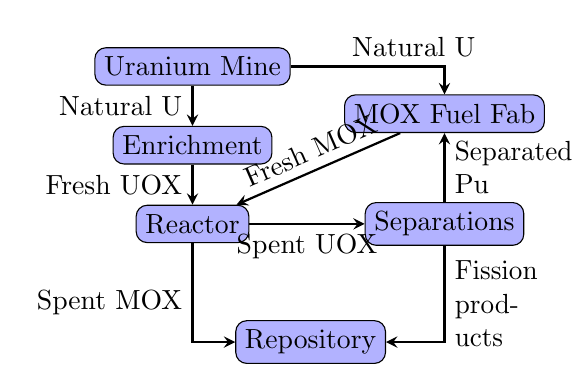
\begin{tikzpicture}[node distance=1cm]
                \node (mine) [facility] {Uranium Mine};
                \node (enrichment) [facility, below of=mine]{Enrichment};
                \node (reactor) [facility, below of=enrichment]{Reactor};
                \node (sinkhlw) [facility, below of=reactor, xshift=1.5cm, yshift=-0.5cm]{Repository};
                \node (separation) [facility, right of=reactor, xshift=2.2cm]{Separations};
                \node (mox_fab) [facility, above of=separation, yshift=0.4cm]{MOX Fuel Fab};
                
                \draw [arrow] (mine) -- node[anchor=east]{Natural U} (enrichment);
                \draw [arrow] (enrichment) -- node[anchor=east]{Fresh UOX}(reactor);
                \draw [arrow] (reactor) -- node[anchor=north]{Spent UOX}(separation);
                \draw [arrow] (separation) -- node[anchor=west, text width=0.5cm]{Separated Pu}(mox_fab);
                \draw [arrow] (separation) |- node[anchor=west, text width=0.5cm, pos=0.3]{Fission products}(sinkhlw);
                \draw [arrow] (mine) -| node[anchor=south, pos=0.4]{Natural U} (mox_fab);
                \draw [arrow] (reactor) |- node[anchor=east, pos=0.3]{Spent MOX} (sinkhlw);
                \draw [arrow] (mox_fab) -- node[anchor=south, sloped]{Fresh MOX} (reactor);
                \end{tikzpicture}
            \caption{Fuel cycle facilities and material flow between facilities for the 
            sample fuel cycle scenarios used to compare the results of the \Cycamore Reactor 
            and OpenMCyclus DepleteReactor archetypes. }
            \label{fig:comparison}
        \end{figure}
    \end{columns}
\end{frame}

\begin{frame}
    \frametitle{Benchmark Results (I)}
    \begin{columns}
        \column[t]{3.5cm}
        \begin{itemize}
            \item Separated plutonium masses differ because of 
                  different depletion methodologies
        \end{itemize}
        \column[t]{6.5cm}
        \begin{figure}
            \centering 
            \includegraphics[scale=0.45, trim=0 0 0 30,clip]{comparison_pu_cumulative.pdf}
            \caption{Comparison of cumulative separated plutonium in benchmark between 
            OpenMCyclus and \Cycamore \texttt{Reactor}.}
        \end{figure}
    \end{columns}
\end{frame}

\begin{frame}
    \frametitle{Benchmark Results (I)}
    \begin{columns}
        \column[t]{3.5cm}
        \begin{itemize}
            \item Separated plutonium masses differ because of 
                  different depletion methodologies
            \item Temporarily changing OpenMCyclus method to better 
                  match with \Cycamore shows better agreement
        \end{itemize}
        \column[t]{6.5cm}
        \begin{figure}
            \centering 
            \includegraphics[scale=0.45, trim=0 0 0 30,clip]{comparison_pu_cumulative_discharge.pdf}
            \caption{Comparison of cumulative separated plutonium in benchmark between 
            OpenMCyclus and \Cycamore \texttt{Reactor}.}
        \end{figure}
    \end{columns}
\end{frame}

\begin{frame}
    \frametitle{Benchmark Results (II)}
        \begin{itemize}
            \item Differences in separated plutonium masses 
                  propagate into different fuel receipts 
            \item Spent fuel masses are mostly consistent, except 
                  when a reactor is decommissioned
        \end{itemize}
        \begin{figure}
            \centering
            \begin{subfigure}{0.48\textwidth}
                \includegraphics[width=\linewidth]{comparison_spentuox.pdf}
                \caption{Comparison of Spent UOX fuel discharged.}
            \end{subfigure}
            \hfill
            \begin{subfigure}{0.48\textwidth}
                \includegraphics[width=\linewidth]{comparison_spentmox.pdf}
                \caption{Comparison of Spent MOX fuel discharged.}
            \end{subfigure}
            \caption{Spent fuel transactions in OpenMCyclus/\Cycamore benchmark}
            \label{fig:spentfuel_benchmark}
        \end{figure}

\end{frame}

\begin{frame}
    \frametitle{Recycle scenario definitions}
    \begin{table}[ht]
        \centering
        \caption{Summary of the recycle fuel cycle transition scenarios.
        Energy growth is relative to energy from \glspl{LWR} in 2025.}
        \label{tab:scenarios_recycle}
        \begin{tabular}{c l l l}
            \hline
            Scenario & Advanced Reactors & Energy demand & Recycle scheme\\\hline
            \rowcolor{lightorange}14 & Xe-100, MMR, VOYGR & No growth & Limited \\
            \rowcolor{lightorange}15 & Xe-100, MMR, VOYGR & No growth & Limited, no TRISO\\
            \rowcolor{lightorange}16 & SFR& No growth & Continuous \\
            \rowcolor{lightpink}17 & Xe-100, MMR, VOYGR & 1\% growth & Limited \\
            \rowcolor{lightpink}18 & Xe-100, MMR, VOYGR & 1\% growth & Limited, no TRISO\\
            \rowcolor{lightpink}19 & SFR & 1\% growth & Continuous\\
            \hline
    \end{tabular}
    \end{table}
        %<2-> \tikz[overlay, remember picture]{\draw{draw=red,thick, double, fillopacity=0.2] ($(infrastructure)+(-0.5,0.4)$) rectangle ($(infrastructure)+(6,-0.2)$);}} 
\end{frame}

\begin{frame}
    \frametitle{Recycle scenario definitions}
        \begin{table}[ht]
            \centering
            \caption{Summary of the recycle fuel cycle transition scenarios.
            Energy growth is relative to energy from \glspl{LWR} in 2025.}
            \label{tab:scenarios_recycle}
            \begin{tabular}{c l l l}
                \hline
                Scenario & Advanced Reactors & Energy demand & Recycle type\\\hline
                \rowcolor{lightorange}\marktopleft{a3}14 & Xe-100, MMR, VOYGR & No growth & Limited \\
                \rowcolor{lightorange}15 & Xe-100, MMR, VOYGR & No growth & Limited, no TRISO\\
                \rowcolor{lightorange}16 & SFR& No growth & Continuous \markbottomright{a3}\\
                \rowcolor{lightpink}17 & Xe-100, MMR, VOYGR& 1\% growth & Limited \\
                \rowcolor{lightpink}18 & Xe-100, MMR, VOYGR & 1\% growth & Limited, no TRISO\\
                \rowcolor{lightpink}19 & SFR & 1\% growth & Continuous\\
                \hline
        \end{tabular}
        \end{table}
\end{frame}




\begin{frame}
    \frametitle{Limited recycle fuel cycle assumptions}
    \begin{columns}
        
    \column[t]{6cm}
    %\vspace{-0.9cm}
    \begin{figure}
    \centering
    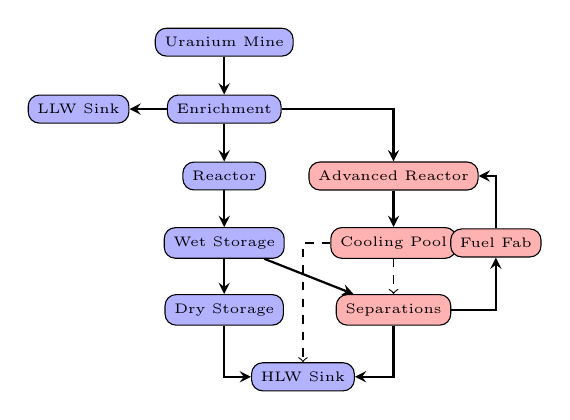
\begin{tikzpicture}[node distance=0.85cm]
        \node (mine) [facility] {\tiny Uranium Mine};
        \node (enrichment) [facility, below of=mine]{\tiny Enrichment};
        \node (reactor) [facility, below of=enrichment]{\tiny Reactor};
        \node (adv_reactor) [transition, right of=reactor, xshift=1.3cm]{\tiny Advanced Reactor};
        \node (wetstorage) [facility, below of=reactor]{\tiny Wet Storage};
        \node (drystorage) [facility, below of=wetstorage]{\tiny Dry Storage};
        \node (cooling) [transition, below of=adv_reactor]{\tiny Cooling Pool};
        \node (sinkhlw) [facility, below of=drystorage, xshift=1cm]{\tiny HLW Sink};
        \node (sinkllw) [facility, left of=enrichment, xshift=-1cm]{\tiny LLW Sink};
        \node (separation) [transition, below of=cooling]{\tiny Separations};
        \node (fuelfab) [transition, below of=adv_reactor,xshift=1.3cm]{\tiny Fuel Fab};
        
        \draw [arrow] (mine) --(enrichment);
        \draw [arrow] (enrichment) -- (reactor);
        \draw [arrow] (enrichment) -- (sinkllw);
        \draw [arrow] (enrichment) -| (adv_reactor);
        \draw [arrow] (reactor) -- (wetstorage);
        \draw [arrow] (wetstorage) -- (drystorage);
        \draw [arrow] (drystorage) |- (sinkhlw);
        \draw [arrow] (adv_reactor) -- (cooling);
        \draw [dashed, ->] (cooling) -- (separation);
        \draw [arrow] (separation) -| (fuelfab);
        \draw [arrow] (fuelfab) |- (adv_reactor);
        \draw [arrow] (separation) |- (sinkhlw);
        \draw [arrow] (wetstorage) -- (separation);
        \draw [dashed, ->] (cooling) -| (sinkhlw);

        \end{tikzpicture}
    \caption{Fuel cycle facilities and material flow between facilities for the recycling 
    scenarios.}
    \label{fig:limited_fuel_cycle}
\end{figure}

        \column[t]{4.5cm}
        \begin{itemize}
            \item Separations start in 2020
            \item U-based fuel is reprocessed, Pu-based fuel is disposed
            \item Reactors prefer Pu-based fuel over U-based fuel
            \item Separations remove Pu
            \item<2-> Use the same deployment schedule as Scenarios 7, 13
            \item<2-> Modeled Xe-100 and VOYGR with OpenMCyclus
            \item<2-> Calculate MOX compositions based on plutonium
                      equivalence
            \item<3-> Assume natural uranium is enriched to produce  
                  fuel
        \end{itemize}

\end{columns}
\end{frame}

\begin{frame}
    \frametitle{Continuous recycle fuel cycle assumptions}
    \begin{columns}
        
    \column[t]{6cm}
    %\vspace{-0.5cm}
    \begin{figure}
    \centering
    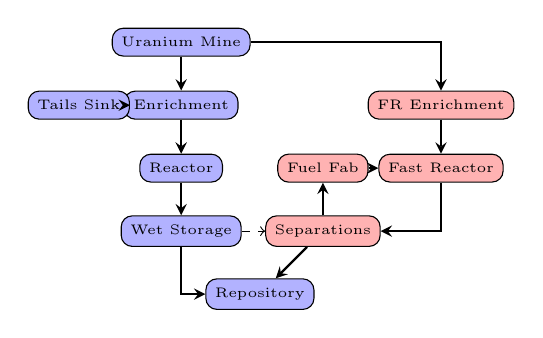
\begin{tikzpicture}[node distance=0.8cm]
        \node (mine) [facility] {\tiny Uranium Mine};
        \node (enrichment) [facility, below of=mine]{\tiny Enrichment};
        \node (reactor) [facility, below of=enrichment]{\tiny Reactor};
        \node (wetstorage) [facility, below of=reactor]{\tiny Wet Storage};
        \node (sinkhlw) [facility, below of=wetstorage, xshift=1cm]{\tiny Repository};
        \node (sinkllw) [facility, left of=enrichment, xshift=-0.5cm]{\tiny Tails Sink};
        \node (separation) [transition, right of=wetstorage,xshift=1cm]{\tiny Separations};
        \node (fuelfab) [transition, above of=separation]{\tiny Fuel Fab};
        \node (fr_enrichment) [transition, right of=enrichment,xshift=2.5cm]{\tiny FR Enrichment};
        \node (sfr) [transition, below of=fr_enrichment]{\tiny Fast Reactor};
        
        \draw [arrow] (mine) -- (enrichment);
        \draw [arrow] (mine) -| (fr_enrichment);
        \draw [arrow] (enrichment) -- (reactor);
        \draw [arrow] (enrichment) -- (sinkllw);
        \draw [arrow] (reactor) -- (wetstorage);
        \draw [arrow] (wetstorage) |- (sinkhlw);
        \draw [arrow] (separation) -- (fuelfab);
        \draw [arrow] (separation) -- (sinkhlw);
        \draw [arrow] (fuelfab) -- (sfr);
        \draw [dashed, ->] (wetstorage) -- (separation);
        \draw [arrow] (sfr) |- (separation);
        \draw [arrow] (fr_enrichment) -- (sfr);

        \end{tikzpicture}
    \caption{Fuel cycle facilities and material flow between facilities for 
    the continuous recycling scenarios.}
    \label{fig:continuous_fuel_cycle}
\end{figure}

        \column[t]{4.5cm}
        \begin{itemize}
            \item Introduce a \gls{SFR} for transition, modeled through 
                  OpenMCyclus
            \item Separation start 2020
            \item Can accept U/TRU fuel (preferred) or \gls{HALEU}
            \item Separations remove U, Np, Pu, Am
            \item<2-> Use the same deployment scheme for the \gls{SFR}
            \item<2-> Calculate \gls{HALEU} composition based on plutonium
                      equivalence
            \item<3-> Assume natural uranium is enriched to produce 
                  fuel
        \end{itemize}

\end{columns}
\end{frame}

\begin{frame}
    \frametitle{Advanced reactors}
    \vspace{-0.7cm}
    \begingroup
        \renewcommand{\arraystretch}{1.5}
        \begin{table}
            \centering
            \begin{threeparttable}
        
            \caption{Fast reactor design specification.}
            \label{tab:fast_rx}
            \begin{tabular}{l l}
                \hline
                Design Criteria & SFR \cite{fichtlscherer_assessing_2019,triplett_prism:_2012}\\
                \hline
                Power Output (MWth) & 840 \\
                Power Output (MWe) & 311 \\
                Capacity Factor & 90\%\tnote{1} \\
                Enrichment (wt\% fissile Pu) &  11.3/13.5\\
                Cycle Length (yrs) & 1 \\
                Number of cycles &  4\\
                Fuel form &  Metallic \\
                Discharge fuel burnup (MWd/kg) & 87.51 \\
                Reactor Lifetime (yrs)&  60\\
                \hline
            \end{tabular}
            \begin{tablenotes}
                \item [1] Assumed value
            \end{tablenotes}
        \end{threeparttable}
        \end{table} 
    \endgroup
\end{frame}

\subsection{Recycle results}

\begin{frame}
    \frametitle{Recycling scheme dictates amount of separated material}
    \begin{itemize}
        \item Scenario 16 (Continuous reprocessing) has the 
              most separated material 
        \item Scenario 15 (Limited, no TRISO) has the least separated 
              material
    \end{itemize}
    \begin{figure}
        \centering
        \begin{subfigure}{0.48\textwidth}
            \includegraphics[width=\linewidth]{nogrowth_recycle_sep_pu.pdf}
            \caption{U-based fuel mass}
        \end{subfigure}
        \hfill
        \begin{subfigure}{0.48\textwidth}
            \includegraphics[width=\linewidth]{nogrowth_recycle_sep_pu_cumulative.pdf}
            \caption{Pu-based fuel mass}
        \end{subfigure}
        \caption{Fuel masses for advanced reactors in Scenarios 14-16}
        \label{fig:recycle_sep_pu}
    \end{figure}
\end{frame}

\begin{frame}
    \frametitle{Recycling decreases HALEU needs}
    \begin{itemize}
        \item Scenario 15 (Limited, no TRISO) requires the most 
              enriched uranium, has least Pu-based fuel
        \item Scenario 16 (Continuous reprocessing) doesn't 
              require any enriched uranium, most Pu-based fuel
    \end{itemize}
    \begin{figure}
        \centering
        \begin{subfigure}{0.48\textwidth}
            \includegraphics[width=\linewidth]{nogrowth_recycle_Uaverages.pdf}
            \caption{U-based fuel mass}
        \end{subfigure}
        \hfill
        \begin{subfigure}{0.48\textwidth}
            \includegraphics[width=\linewidth]{nogrowth_recycle_MOX.pdf}
            \caption{Pu-based fuel mass}
        \end{subfigure}
        \caption{Fuel masses for advanced reactors in Scenarios 14-16}
        \label{fig:recycle_fuel}
    \end{figure}
\end{frame}
\section{Sensitivity analysis \& Optimization}
\subsection{Sensitivity analysis}
\begin{frame}
    \frametitle{Sensitivity analysis provides more insight into 
    the fuel cycles.}
    To meet the third objective, I perform sensitivity analysis 
    on Scenario 7, comparing the impact of different model parameters
    \begin{itemize}
        \item Couple \Cyclus with Dakota \cite{adams_dakota_2021}
        \item Parameters include:
        \begin{itemize}
            \item Transition start time
            \item Percent of \glspl{LWR} operating for 80 years
            \item Build share of Xe-100, VOYGR, MMR
            \item Discharge burnup of Xe-100 and MMR
        \end{itemize}
        \item Vary these parameters individually
        \item Vary these parameters in different combinations
    \end{itemize}

\end{frame}

\begin{frame}
    \frametitle{Varying the Xe-100 build share has a mixed effect}
    \begin{columns}

        \column[t]{4.5cm}
        \begin{itemize}
            \item HALEU-related metrics all increase
            \item Total fuel mass and the SNF mass decrease
            \item Total SWU capacity is relatively constant
            \item Results are a function of the number of
                  each advanced reactor deployed
        \end{itemize}

    \column[t]{5.5cm}
    \begin{figure}
        \centering 
            \includegraphics[scale=0.4]{xe100.pdf}
            \caption{Relative effect of varying Xe-100 build share}
            \label{fig:xe100_effects}
    \end{figure}

\end{columns}
\end{frame}

\begin{frame}
    \frametitle{Effects of varying Xe-100 build share}
    \begin{figure}
        \centering
        \includegraphics[scale=0.5]{xe100_combined_reactors.pdf}
        \caption{Number of Xe-100s (top left), MMRs (top right), and VOYGRs
        (bottom left) as a function of Xe-100 build share.}
        \label{fig:xe100_s7_combined_reactors}
    \end{figure}
\end{frame}

\begin{frame}
    \frametitle{Effects of varying Xe-100 and MMR burnup}
    \begin{columns}

        \column[t]{4cm}
        \begin{itemize}
            \item Non-uniform relationship
            \item At smaller Xe-100 burnup values the increasing MMR 
                  share decreases the HALEU mass
            \item At larger Xe-100 burnup values the increasing MMR share 
                  increases the HALEU mass
            \item Comparison of how much fuel each reactor needs
        \end{itemize}

    \column[t]{6cm}
    \vspace{-1cm}
    \begin{figure}
        \centering 
            \includegraphics[scale=0.5, trim=180 45 70 50,clip]{mmr_share_xe100_burnup_haleu.pdf}
            \caption{Effects of varying the MMR build share and 
            Xe-100 discharge burnup on HALEU mass}
            \label{fig:mmr_share_xe100_bu}
    \end{figure}

\end{columns}
\end{frame}

\begin{frame}
    \frametitle{Varying multiple parameters shows importance of the 
    Xe-100 burnup}
    \begin{table}
        \centering
        \caption{Sobol' indices for the Gaussian model when varying the 
        Xe-100 build share. Highlighted 
        values indicate a total Sobol' indices of above 0.5.}
        \label{tab:s7_sobol_xe100_gaussian}
        \begin{tabular}{c c c c c c c}
            \hline
            & \multicolumn{6}{c}{Output Metric} \\
            Parameter & Fuel Mass & HALEU Mass & SWU & HALEU SWU & Feed & SNF Mass \\
            \hline
            Transition Start & 0.003 & 0.007 & 0.009 &
                               0.009 & 0.009 & 0.003\\
            LWR Lifetime & 0.280 & 0.021 & 0.095 &
                           0.022 & 0.022 & 0.314\\
            Xe-100 Share & \cellcolor{green!25}0.533 & \cellcolor{green!25}0.513 & 0.283 &
            \cellcolor{green!25}0.511 & \cellcolor{green!25}0.512 & 0.474\\
            Xe-100 Burnup & 0.247 & \cellcolor{green!25}0.571 & \cellcolor{green!25}0.775 & 
            \cellcolor{green!25}0.568 & \cellcolor{green!25}0.568 & 0.280\\
            MMR Burnup & 0.002 & 0.004 & 0.006 & 
                         0.005 & 0.005 & 0.002\\
            \hline        
        \end{tabular}
    \end{table}
        %<2-> \tikz[overlay, remember picture]{\draw{draw=red,thick, double, fillopacity=0.2] ($(infrastructure)+(-0.5,0.4)$) rectangle ($(infrastructure)+(6,-0.2)$);}} 
\end{frame}

\subsection{Optimization}
\begin{frame}
    \frametitle{Use the \Cyclus-Dakota coupling to optimize the transition}
    \begin{itemize}
        \item Use the Genetic algorithm in Dakota (single-objective or 
        multi-objective) to perform optimization.
        \item Use the parameters considered for sensitivity analysis, 
              except the transition start time
        \item Apply a linear constraint for the advanced reactor build shares
        \item Goal is to minimize the SWU capacity needed to 
             produce HALEU, the mass of SNF, or both
    \end{itemize}
\end{frame}

\begin{frame}
    \frametitle{Multi-objetive optimization isn't perfect}
    \begin{columns}
        \column[t]{5cm}
        \begin{itemize}
            \item Optimizing for these metrics is a trade-off between 
                 building Xe-100s and VOYGRs
            \item Genetic algorithm struggles with linear constraint for 
                  the three build shares
        \end{itemize}

        \column[t]{5cm}
        \begin{figure}
            \centering 
            \includegraphics[scale=0.4]{once_through_pareto.pdf}
            \caption{Pareto front for multi-objective optimization}
            \label{fig:pareto}
        \end{figure}
    \end{columns}
    
\end{frame}
\section{Effects of impurities}
\begin{frame}
    \frametitle{Downblending HEU is a potential source of HALEU}
    To meet the fourth objective, I modeled the neutronics of 
    different HALEU compositions in the Xe-100 and MMR.
    \begin{itemize}
        \item Consider pure HALEU ($^{235}$U and $^{238}$U only)
              and HALEU from downblended \gls{EBR} 
              \cite{vaden_isotopic_2018} and Y-12 
              \cite{nelson_foreign_2010} stockpiles
        \item Create models in Serpent \cite{leppanen_serpent_2013} 
              for these two reactors
        \item Compare the performance of the fuels with respect to:
        \begin{itemize}
            \item \keff
            \item \betaEff
            \item Energy- and spatially-dependent flux
            \item Fuel, coolant, moderator, and total reactivity
                  temperature feedback coefficients
        \end{itemize}
    \end{itemize}

\end{frame}

\begin{frame}
    \frametitle{Energy dependent neutron flux in Xe-100}
    \begin{figure}
        \centering 
        \includegraphics[scale=0.5]{xe100_mg_flux.pdf}
        \caption{Energy-dependent flux through the active region 
        of the Xe-100 core. The purple line is the delineation 
        between fast and thermal neutrons for this work.}
    \end{figure}
\end{frame}

\begin{frame}
    \frametitle{Spatitally-dependent neutron flux in Xe-100}
    \begin{figure}
        \centering 
        \begin{subfigure}{0.49\textwidth}
            \includegraphics[scale=0.35, trim=20 10 10 20,clip]{xe100_thermal_radial.pdf}
        \end{subfigure}
        \begin{subfigure}{0.49\textwidth}
            \includegraphics[scale=0.35, trim=10 10 10 20,clip]{xe100_fast_radial.pdf}
        \end{subfigure}
        \caption{Radial fluxes through Xe-100.}
        \label{fig:xe100-flux}
    \end{figure}
\end{frame}
\section{Conclusions}
% General Summary


The goal of this work is to investigate the impacts of deploying reactors 
fueled 
by \gls{HALEU} in the United States, including the impacts that the reactors 
have on the \gls{NFC} and the impacts the \gls{NFC} has on the reactors. 
The results of this work are intended to
aid and guide policy makers and key stake holders on how to best establish a 
fuel cycle to support the deployment of \gls{HALEU}-fueled reactors. 
Within this primary goal, there are three specific objectives:
\vspace{0.2cm} 
\noindent
\begin{enumerate}
\item Quantify potential material requirements for the transition 
from \glspl{LWR} to advanced reactors in open and closed 
fuel cycles.

\item Understand the impacts of fuel cycle parameters on the material 
requirements and design optimized transition scenarios.

\item Identify potential limitations in using downblended \gls{HEU} 
on reactor performance.

\end{enumerate}

These goals were met by designing and modeling various transitions 
to advanced reactors, considering a once-through and a closed 
fuel cycle. The once through fuel cycles were then investigated 
further by performing sensitivity analysis and optimization. Finally, 
models of two different \gls{HALEU}-fueled advanced reactors were 
created to investigate the impact of different uranium isotopic 
compositions of the \gls{HALEU} fuel on reactor performance. 

% Once-through analysis

% Closed fuel cycle analysis

% Sensitivity analysis
Chapter 6 examined the effects of different input parameters for 
their effects on different output metrics for the fuel cycle transition from 
\glspl{LWR} to different advanced reactors. The \gls{OAT} analysis identified the 
trends from varying each input parameter independently, and how the deployment 
scheme for this work impacts each of the results. The analysis also 
identified tradeoffs between different reactor designs, such as how the Xe-100 
needs more \gls{HALEU} than the VOYGR, but a smaller fuel mass. The synergistic 
analysis identified how some of the input parameters interact to affect the output 
metrics. While some of the combinations of input parameters (e.g., varying 
the \gls{LWR} lifetime and the VOYGR build share) had consistent trends 
across the input parameter space, some combinations (e.g., varying the Xe-100 
burnup and the \gls{MMR} share) varied in their effect across the input parameter 
space. Finally, the global sensitivity analysis quantified the effect of different 
input parameters on the output metrics. We build surrogate models to fully capture 
the input parameter space. The models were consistent with the Sobol' indices, 
such that the Xe-100 burnup is the most impactful parameter when varying any 
of the three advanced reactor build shares. 

% Optimization
Chapter 7 demonstrated a methodology to optimize the once-through 
transitions and identified transitions that minimize different 
fuel cycle metrics. Results from this chapter show that minimizing the 
\gls{SWU} capacity to produce \gls{HALEU} requires maximizing the number of 
VOYGRs built, minimizing the mass of \gls{SNF} requires maximizing the number 
of Xe-100s built, and minimizing both of these fuel cycle metrics is a 
balance between deploying Xe-100s and VOYGRs. The results from the optimization 
work was consistent with the results of the sensitivity analysis, but 
they did not fully meet expectations. The input parameters identified that 
were not subject to a linear constraint (i.e., not the advanced reactor 
build shares) matched expectations based on the trends of the sensitivity 
analysis and intuition. However, The methodology employed for this 
analysis did not adhere well to the linear constraint of the advanced reactor 
build shares in all three of the problems. Therefore, the 
results from the optimization work can not be taken at face value 
and are better used to identifying a relationship between the advanced 
reactor build shares than a specific set of parameters. 


% Neutronics
 
\section{Future Work}
The work performed here provides a foundation for continued analysis and 
exploration of the fuel cycle impacts of deploying \gls{HALEU}-fueled reactors. 
Potential areas of future work include modeling non-fuel materials needed 
to support these transitions, such as the amount of reactor-grade graphite 
to be the moderators in the Xe-100 and \gls{MMR}. This analysis would 
provide insight into other supply chain requirements that equally 
impactful on establishing these fuel cycles. Additionally, the 
results of this work can be used to determine facility sizes, throughputs, 
and numbers. This information aids in developing the supply chains 
to support these transitions, but also in designing and evaluating 
safeguards for these transitions. Potential safeguards measures may 
limit the facility sizes and the amount of material that can move from 
one facility to another, which affects how the transition can be 
implemented. By 
incorporating facility information into the fuel cycle model, the 
sensitivity analysis and optimization methodologies can be used 
to identify ways to adjust the transition to better account for 
the facility limitations and safeguards needs. 

The analysis of the downblended \gls{HEU} on the reactor performance
can also be expanded. For example, consider other \gls{HALEU}-fueled 
reactors, such as the Oklo Aurora, that have announced an intent to 
use \gls{HALEU} created from these stockpiles. Additionally, expand 
the analysis to other metrics, such as power peaking factors and 
power distributions in the core, or 
increase the fidelity of the models. Ways to increase the model 
fidelities include incorporating burnable poisons, control rods, 
and couple with heat transfer calculations to create a multi-physics model. 
These incorporations into the models will provide greater 
accuracy to the results. 
\begin{frame}
    \frametitle{Acknowledgements}
    This material is based upon work supported under a University 
    Nuclear Leadership Program Graduate Fellowship. Any opinions, findings, conclusions, or 
recommendations expressed in this publication are those of the author(s) 
and do not necessarily reflect the views of the Department of Energy Office 
of Nuclear Energy.

\end{frame}


\begin{frame}[allowframebreaks]
    \frametitle{References}
    \bibliographystyle{plain}
    {\footnotesize \bibliography{../bibliography} }
  
\end{frame}

\begin{frame}
    \centering
    \includegraphics[scale=0.25,trim=0 600 0 700,clip]{LittleR.jpg}
\end{frame}

\begin{frame}
    \frametitle{Once-through feed uranium}
    \begin{figure}
        \centering 
        \includegraphics[scale=0.5]{nogrowth_feed.pdf}
    \end{figure}
\end{frame}

\begin{frame}
    \frametitle{Recycle HLW}
    \begin{figure}
        \centering
        \includegraphics[scale=0.5]{nogrowth_recycle_hlw.pdf}
    \end{figure}
\end{frame}

\begin{frame}
    \frametitle{Recycle SNF}
    \begin{figure}
        \centering
        \includegraphics[scale=0.3]{nogrowth_recycle_snf.pdf}
    \end{figure}
\end{frame}

\begin{frame}
    \frametitle{Recycle SWU}
    \begin{figure}
        \centering
        \includegraphics[scale=0.3]{nogrowth_recycle_swu.pdf}
    \end{figure}
\end{frame}

\begin{frame}
    \frametitle{Effects of varying VOYGR build share}
    \begin{figure}
        \centering
        \includegraphics[scale=0.5]{voygr.pdf}
    \end{figure}
\end{frame}

\begin{frame}
    \frametitle{Effects of varying MMR build share}
    \begin{figure}
        \centering
        \includegraphics[scale=0.3]{mmr.pdf}
    \end{figure}
\end{frame}

\begin{frame}
    \frametitle{Axial flux through Xe-100}
    \begin{figure}
        \centering 
        \begin{subfigure}{0.49\textwidth}
            \includegraphics[scale=0.35, trim=20 10 10 20,clip]{xe100_thermal_axial.pdf}
        \end{subfigure}
        \begin{subfigure}{0.49\textwidth}
            \includegraphics[scale=0.35, trim=10 10 10 20,clip]{xe100_fast_axial.pdf}
        \end{subfigure}
        \caption{Axial fluxes through Xe-100.}
        \label{fig:xe100-axial-flux}
    \end{figure}
\end{frame}

\begin{frame}
    \frametitle{Reactivity feedback coefficients for Xe-100}
    \begin{table}[ht]
        \centering
        \caption{Reactivity temperature feedback coefficients for 
        each material type in the Xe-100-like model for each fuel 
        type.}
        \label{tab:coeff_xe100}
        \begin{tabular}{c c c c c}
            \hline 
            & \multicolumn{4}{c}{Material feedback coefficient (pcm/K)} \\
            Fuel Type & Fuel & Coolant & Moderator & Total \\
            \hline
            Pure & -3.875 $\pm$ 0.094 & -0.044 $\pm$ 0.112 & -0.071 $\pm$ 0.459 & -4.216 $\pm$ 0.502\\
            \gls{EBR} & -3.759 $\pm$ 0.138 & -0.433 $\pm$ 0.048 & -0.708 $\pm$ 0.404 & -4.817 $\pm$ 0.438\\
            Y-12 & -3.797 $\pm$ 0.157 & -0.351 $\pm$ 0.092 & -0.728 $\pm$ 0.469 & -4.700 $\pm$ 0.349\\
            \hline

        \end{tabular}
\end{table}
\end{frame}

\end{document}
